\documentclass[letterpapaer]{article}

\usepackage{geometry}
\usepackage{mathtools}
\usepackage{amsmath}
\usepackage{amsfonts}
\usepackage{epstopdf}
\usepackage{graphicx}
\usepackage{multirow}
\usepackage{engord}
\usepackage{url}
\usepackage{hyperref}
\usepackage{indentfirst}
\usepackage{abstract}

\renewcommand{\abstractnamefont}{\normalfont\Large\bfseries}

\usepackage{setspace}
\setlength{\lineskiplimit}{10pt}
\setlength{\lineskip}{5pt}

\newcommand{\HRule}{\rule{\textwidth}{0.7mm}}

\bibliographystyle{plain}

\title{STATS 503 Final Project:\\Precipitation Prediction}
\author{Shengchen Hao, Ruikun Xiao, Zetan Li}
\date{April.11, 2018}

\begin{document}
\begin{titlepage}
\begin{center}
\HRule \\[0.4cm]
{ \huge \bfseries STATS 503 Final Project:\\ Precipitation Prediction}\\[0.2cm]
\HRule \\[0.6cm]
{ \Large \bfseries Shengchen Hao, Ruikun Xiao, Zetan Li}\\[0.4cm]
{ \large \bfseries University of Michigan}\\[1.0cm]
\end{center}

 \vspace{1cm}

\begin{abstract}
\large

Daily climate data of Seattle are used to establish models to predict precipitation in the following day. With new variables constructed to improve model performance, three different algorithms are applied to the dataset: random forest, support vector machine and $k$-nearest neighbors. The models' performances on the test set and daily climate data of New York City are respectively checked and compared.

\end{abstract}

 \vspace{3cm}

\section*{Contributions}

\large

 \vspace{0.5cm}

\noindent \textbf{Shengchen Hao: }1, 2.2-3, 3.1-2, 4.2, 4.5, 5\\

\noindent \textbf{Ruikun Xiao: }Abstract, 2.1, 3.3-4, 4.1, 4.4, \LaTeX\\

\noindent \textbf{Zetan Li: }1, 2.1, 4.3, 4.5, 5

\end{titlepage}
\tableofcontents
\section{Introduction}

Weather forecast is important for people to make their schedule for the next day. Among those technical terms in the forecasting, temperature and precipitation are the most important for the public. Nowadays weather forecasts, especially the precipitation forecast is conducted with the help of satellite images of clouds. This requires knowledge in meteorology. So we wonder if we can predict whether it will rain tomorrow based on the basic weather record (like temperature, precipitation, wind), with the classification method we learned in class.

We choose Seattle for our study as it usually has half of time in a year raining, so the data are balanced. In order to make better forecasting, feature engineering is needed. Also the data comes in form of daily report by each station. Combining the weather report each day from different stations is also a challenge for our study.  The location of weather stations and relationship between variables are discussed in the section of data exploration. And we are going to use Random Forest, $k$-NN and SVM for classification. At last part we are going to use the models trained with Seattle data to predict precipitation in another city to see whether the models are generally usable.
\section{Data Exploration}
\subsection{Dataset in Use}

The dataset used in our study is obtained from \href{https://www.ncdc.noaa.gov/cdo-web/}{NOAA} (National Oceanic and Atmospheric Administration). It is a part of NOAA's GHCN(Global Historical Climatology Network)-Daily database\cite{noaa}, and is concerned with daily climate data of Seattle from January \engordnumber{1}, 2012 to January \engordnumber{1}, 2018. The records are colloected from up to 190 stations accross Seattle area, with different sets of attributes. The main attributes are listed in Table \ref{tbld}.

For practical use, we sample $70\%$ of the data as the training set, and the rest as the test set.

The models are also applied to daily climate data of New York in 2017, which come from the same database.

\begin{table}[h]
\setlength{\belowcaptionskip}{5pt}
\caption{Attributes of the Dataset}
\label{tbld}
\centering
\renewcommand\arraystretch{1.5}
\begin{tabular}{|c|l|}
\hline
\textbf{Attribute} & \textbf{Explanation (unit)}\\
\hline
PRCP & Precipitation (inches)\\
\hline
TMAX & Maximum temperature ($^\circ$F)\\
\hline
TMIN & Minimum temperature ($^\circ$F)\\
\hline
TOBS & Temperature at the time of observation ($^\circ$F)\\
\hline
WDF2 & Direction of fastest 2-minute wind ($^\circ$)\\
\hline
WDF5 & Direction of fastest 5-second wind ($^\circ$)\\
\hline
WSF2 & Fastest 2-minute wind speed (miles/h)\\
\hline
WSF5 & Fastest 5-second wind speed (miles/h)\\
\hline
AWND & Average daily wind speed (miles/h)\\
\hline
\end{tabular}
\end{table}
\subsection{Distribution of Weather Stations}

It is provided with the original dataset the positions of the weather stations across Seattle (in longitude, latitude and elevation), which is important as Seattle is surrounded by mountains and the weather records may vary a lot due to geographic differences.

The two maps in Figure \ref{pos} is constructed with weather records in a particular day. The colors of points in the map indicate the values of different variables, and the grey points represent values not recorded (missing). As shown in left hand side, the south part of Seattle precipitated and the north part didn't. Also there are 3 stations at the east of Seattle city recorded high precipitation, which located in Mt Rainier. The max temperature records also vary a lot between downtown Seattle and mountains around. So it is important to find a threshold of PRCP to decide whether it rained in Seattle that day. Also to mention that the stations are randomly distributed across Seattle area and shows no clustering pattern. Therefore, it is no point to perform clustering on stations' location.

\begin{figure}[h]
\centering
\begin{minipage}[t]{0.48\textwidth}
\centering
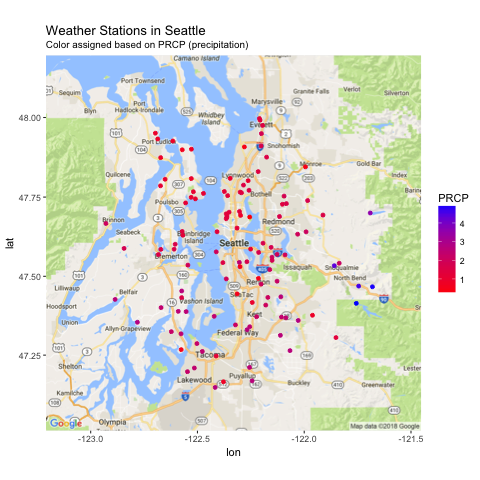
\includegraphics[width=6cm]{station1.png}
\end{minipage}
\begin{minipage}[t]{0.48\textwidth}
\centering
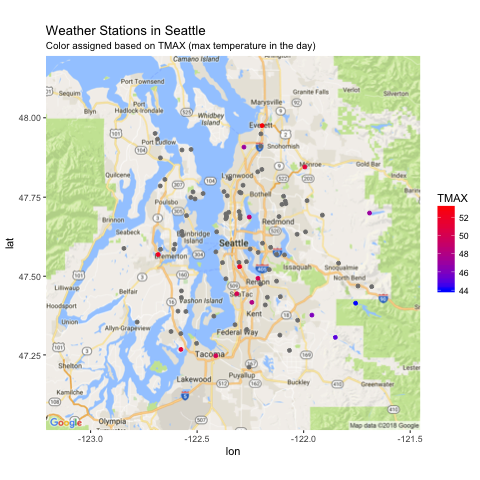
\includegraphics[width=6cm]{station2.png}
\end{minipage}
\caption{Station Positions}
\label{pos}
\end{figure}
\subsection{Missing Value and the Reason to Take Mean}

As we can see, (\expandafter{\romannumeral1}) the attributes recorded by each weather station are quite different, (\expandafter{\romannumeral2}) there are lots of missing values for each day. However, since the time sequence is significantly importance for our study, we can not afford to remove any single row in the data. It is also not feasible to substitute the missing values because of sparsity of the dataset. Instead, since we have records from approximately 100 stations each day, we can take mean of each scalar attribute (temperature, precipitation, etc.), and take weighted mean vector of each vector attribute (attributes related to wind). By doing so we have a row that contains all the attributes for each date, and remove the attributes that still have missing values.

As we can see, the attributes recorded by each weather station are quite different, and there are lots of missing values for each day. However, since the time sequence is significantly importance for our study, we can not afford to remove any single row in the data. It is also not feasible to substitute the missing values because of the sparsity of the dataset. The first way is performing clustering based on the location of stations, substitute missing values with the mean of variables within each cluster. As shown in Figure \ref{clust}, we have the largest average silhouette width when k = 2. The map plot on the right hand side of Figure \ref{clust} shows the clustering result, basically the stations are separated into two clusters, west and east, with downtown Seattle as the boundary in the middle. However, with this method we may create missing values since some of the variables are only recorded by stations in one cluster. Also it is hard to tell the relationship between clusters and the way to combine variables is harder. Therefore, we decided not to use clustering for substituting missing values.
 
Instead, since we have records from approximately 100 stations each day, we can group by date and take mean of each scalar attribute (temperature, precipitation, etc.) directly, and take weighted mean vector of each vector attribute (attributes related to wind). By doing so we have a row that contains all the attributes for each date, and remove the attributes that still have missing values.

\begin{figure}[h]
\centering
\begin{minipage}[t]{0.48\textwidth}
\centering
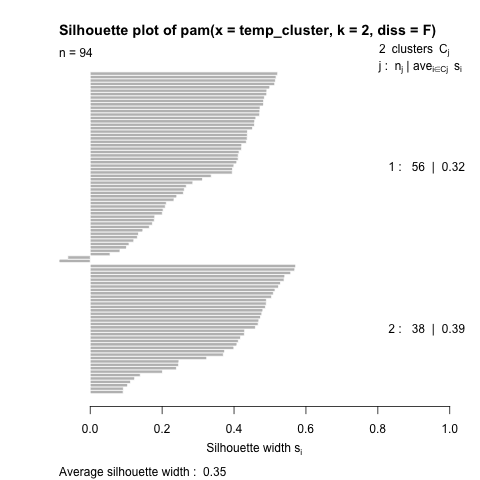
\includegraphics[width=6cm]{silhouette.png}
\end{minipage}
\begin{minipage}[t]{0.48\textwidth}
\centering
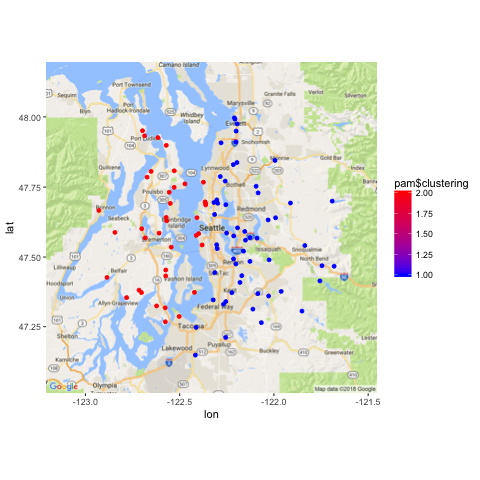
\includegraphics[width=6cm]{clustermap.png}
\end{minipage}
\caption{Clustering Results}
\label{clust}
\end{figure}
\section{Preprocessing}
\subsection{Feature Engineering}

Despite the variables provided by original data, we construct some new variables to improve model performance. As we are trying to forecast whether it would precipitate in the next day, the temperature difference in each day could be important. Rain is formatted by condensation of water in air, higher temperature could contribute to evaporation of water and lower temperature may lead to condensation. Therefore, the temperature differences could be useful in predicting precipitation. 

With TMAX (Max temperature in the day) and TMIN in the original data, we construct TDIF = TMAX - TMIN to measure the temperature difference each day. By looking into TDIF in different days we find some interesting phenomena. The overall TDIF is significantly larger in summer than in winter, which can be seen from the range of TDIF in Figure \ref{tdif}. It is also interesting that TDIF at mountain areas is higher than downtown areas in summer, and right the opposite in winter. Those two phenomena indicate the existence of a seasonal pattern in TDIF, and this could be the same for PRCP.

\begin{figure}[h]
\centering
\begin{minipage}[t]{0.48\textwidth}
\centering
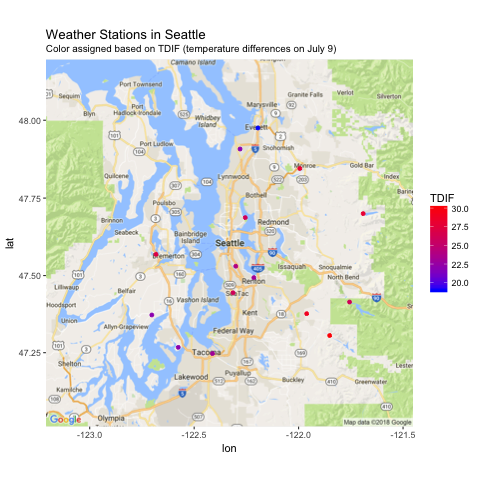
\includegraphics[width=6cm]{tdif1.png}
\end{minipage}
\begin{minipage}[t]{0.48\textwidth}
\centering
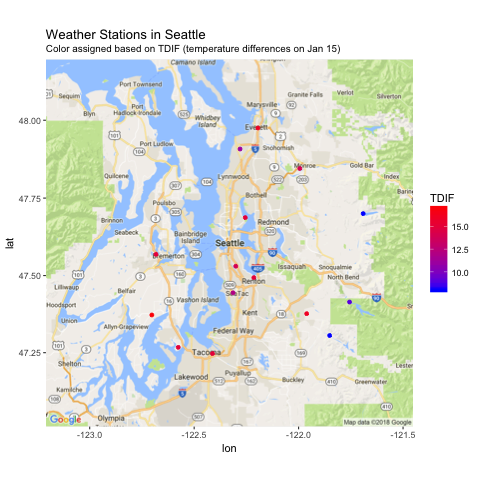
\includegraphics[width=6cm]{tdif2.png}
\end{minipage}
\caption{Stations with TDIF Records}
\label{tdif}
\end{figure}
\subsection{A Short Analysis of Seasonal Pattern in TDIF and PRCP}

Spectrum analysis\cite{priestley1981spectral}, also referred to as frequency domain analysis, is the technical process of decomposing a complex signal into simpler parts. If we consider the time series of TDIF as a signal with a seasonal pattern, we can use the spectrum analysis method to identify the dominant frequency.

First let's see the plot on the left of Figure \ref{patt}. There is an obvious peak in the plot, which is the frequency domain. The cycle corresponding to the peak is 375 days, i.e. TDIF basically follows a cycle of 375 days. And there are no other peaks in the plot, so it indeed is the dominant one.

\begin{figure}[h]
\centering
\begin{minipage}[t]{0.48\textwidth}
\centering
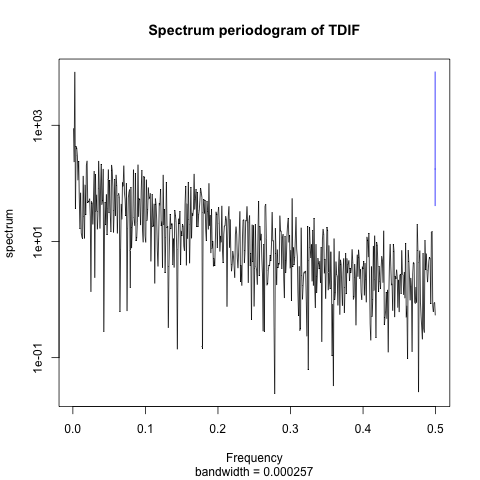
\includegraphics[width=6cm]{patt1.png}
\end{minipage}
\begin{minipage}[t]{0.48\textwidth}
\centering
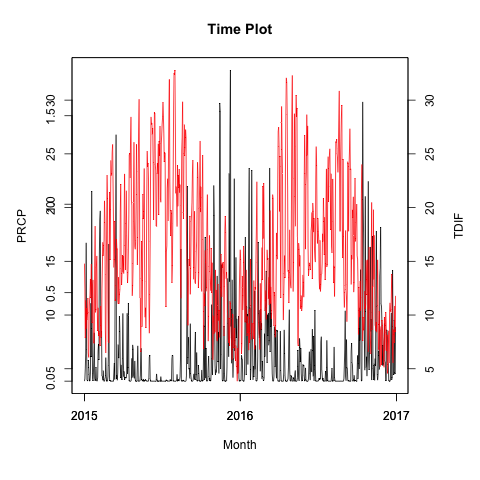
\includegraphics[width=6cm]{patt2.png}
\end{minipage}
\caption{Spectrum Plot and Time Plot}
\label{patt}
\end{figure}

On the right hand side is the time plot of TDIF (the red line) and PRCP (the black line). The red line shows a clear cycle per year, corresponding to the spectrum analysis before. On the other hand, no clear pattern of the black line can be observed. But it can tell us that PRCP is likely to be high when TDIF is low and vice versa. Overall even if we confirm the existence of a seasonal pattern in PRCP (which should be true), it may not play a crucial role in predicting daily weather. However, what we learn from the analysis above is, the TDIF is important in predicting PRCP and they are likely to be not positively, but negatively correlated.
\subsection{Wind Speed and Wind Directions}

As we have mentioned, there are four attributes regarding wind (WSF2, WDF2, WSF5, WDF5) in the data. Among the four, each pair of (WSF, WDF) represents a 2-dim \emph{vector} (wind vector) in polar coordinates. Sometimes, there is a significant variation of directions between different records of the same day, and thus, we shouldn't take their mean directly.

To better summarize the wind vectors, we may consider a natural model about the wind vectors in station $i$:
$$\vec v_i(t)=\vec{v}(t)+\vec u_i+\vec\epsilon_i(t),$$
where $\vec{v_i}(t)$ is the wind vector at station $i$ by time $t$, $\vec u_i$ is a fixed effect for station $i$, and $\vec \epsilon_i(t)$ is the error vector.

With the assumption that the term $\vec\epsilon_i(t)$ has i.i.d. bivariate normal distribution, we may estimate the overall wind vector by estimator
$$\hat{\vec v}_i(t)=\frac1n\sum_{i=1}^n\vec v_i(t)$$
with a constant bias
$$\vec b=\frac1n\sum_{i=1}^n\vec u_i.$$
Such bias here can be viewed as a fixed translation of the attribute space (since it is constant), and can thus be omitted in further analyses.

Since we are only interested in the overall wind condition for Seattle, further analyses would only be concerned with the mean vectors $\hat{\vec v}(t)$. For convenience they are still presented in polar coordinates with the same attribute names. (It might be hard to interpret if they are presented in Cartesian coordinates.)

It is perhaps remarkable that since we have polar coordinates as attributes, the attribute space would not be flat. In fact, the subspace regarding WDF2 (and the one regarding WDF5 as well) is homeomorphic to $\mathbb S^1$ instead of $\mathbb R^1$.
\subsection{Label for Each Day}

Since the data are to be reduced into daily records, there is a problem of determining the labels. For the purpose of our project, we have to assign to every observation (i.e. a specific day) a label representing the weather type of the next day based on precipitation data collected from different stations.

According to the U.S. National Weather Service (NWS), the threshold for daily precipitation is usually 0.01 inches (0.25 mm). With such threshold, we may get daily weather type for every station. It is then natural to let them vote for the daily weather type of the city: a day should be viewed as ``a day with precipitation" if and only if the precipitation recorded are more than 0.01 inches for over half of the stations. To make it clear, a specific day should be labeled according to the proportion of the stations recording more than 0.01 inches of precipitation in following day.

Such labels can be justified by showing that it meets the data from NWS pretty well.\footnote{In fact, the voting threshold, i.e. $50\%$, is also determined by minimizing the RSS (residual sum of squares).}

By applying such labels, we may notice that the data set is quite balanced: there are 974 days with precipitation among the 2192 days observed here.

\begin{figure}[h]
\center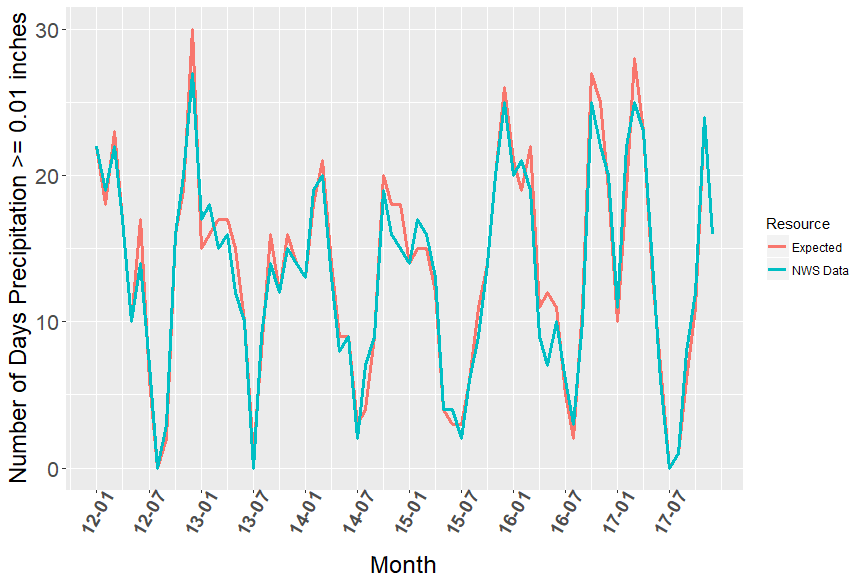
\includegraphics[width = .7\textwidth]{rainyday.png}
\caption{Monthly Number of Days Precipitation \(\geq\) 0.01 Inches}
\label{rainyday}
\end{figure}
\section{Forecasting}
\subsection{Method Selection}

Before establishing models for prediction, we have to choose what algorithms to use in analyses.

Besides common considerations, what we especially take into account is the global topology of the attribute space: because of the attributes WDF2 and WDF5, the space is in fact homeomorphic to $\mathbb R^{p-2}\times \mathbb S^1\times\mathbb S^1$ instead of $\mathbb R^p$. In this case, a hyperplane (or, more generally, an \emph{open} hypersurface) may not be able to seperate it into two \emph{disconnected} subspace.

As the result, we exclude LDA, QDA and several other well-developed classification methods because an open hypersurface is always needed for these. Instead, we tend to apply methods that do not heavily depend on global topology (random forest, $k$-NN) or that classify with a \emph{closed} hypersurface (kernel SVM).
\subsection{Random Forest}

Random forest is an algorithm developed from decision tree. Trees that are grown very deep tend to learn highly irregular patterns: they overfit their training sets. Random forest is a way of averaging multiple deep decision trees, trained on different parts of the same training set, with the goal of reducing the variance. This comes at the expense of a small increase in the bias and some loss of interpretability, but generally greatly boosts the performance in the final model.

The major advantage of random forest is that it is robust against colinearity, and we can rank the importance of variable based on out-of-bag error\cite{breiman2001random}. As it is easy to carry out and require no data assumption, we decided to first run it to get a better idea about which variable is more vital in weather forecast. 

\begin{figure}[h]
\centering
\begin{minipage}[t]{0.48\textwidth}
\centering
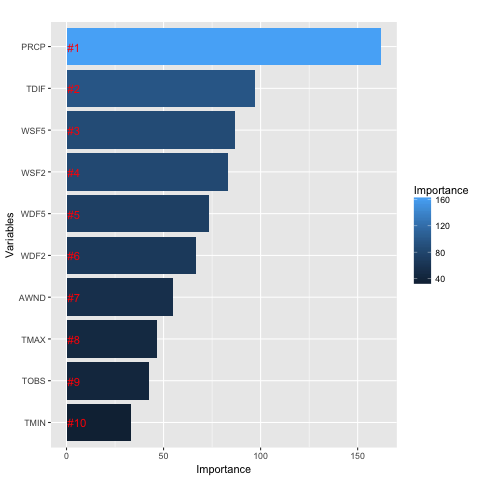
\includegraphics[width = .99\textwidth]{vimp.png}
\caption{Importance of Attributes}
\label{vimp}
\end{minipage}
\begin{minipage}[t]{0.48\textwidth}
\centering
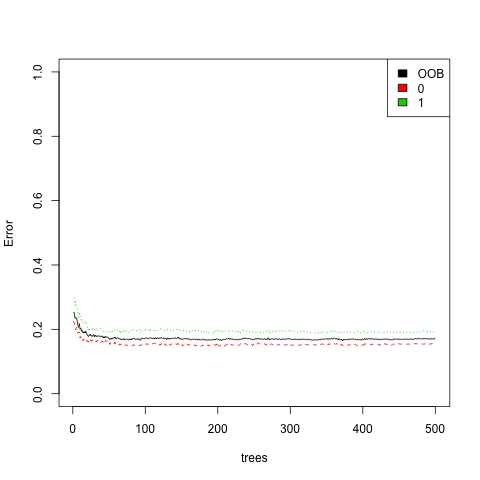
\includegraphics[width = .99\textwidth]{errf.png}
\caption{Error Rate of Random Forest on Training Data}
\label{errf}
\end{minipage}
\end{figure}

As shown in Figure \ref{vimp}, the PRCP is the most important variable. This is intuitively correct as it is the most relative variable. Also we can see our feature engineering plays an important role. The TDIF (temperature difference) and other variables about wind are ranking from \engordnumber{2} to \engordnumber{6}. This give us a sense of what variable should be used in the $k$-NN, since $k$-NN prefers a lower dimension input data.

In Figure \ref{errf}, the error rate become stable when tree number is greater than 100. As the green line is the error rate of predicting days with precipitation and the red line is for days without. The model has a better ability in predicting days without precipitation. This can be numerically confirmed from the confusion matrix in Table \ref{tblrf}. The type \uppercase\expandafter{\romannumeral1} error is higher than type \uppercase\expandafter{\romannumeral2} error, which means the model makes more mistake in predicting days with precipitation. The overall test errors are shown in Table \ref{tblrf}.

Although random forest has many advantages, it still can't deal with the situation when data are not linear separable. So in that case we should try kernel SVM for the next step.

\begin{table}[h]
\setlength{\belowcaptionskip}{5pt}
\caption{Confusion Matrix and Error Rates of Random Forest}
\label{tblrf}
\centering
\renewcommand\arraystretch{1.5}
\begin{tabular}{rrrrr}
\hline
\hline
 & & \multicolumn{2}{c}{True Condition} & \\
\hline
 & & Non-Precipitation & Precipitation & \\
\cline{1-4}
\multirow{2}{*}{Prediction} & {Non-Precipitation} & 339 & 51 & \\
\cline{2-4}
&Precipitation&52&217&\\
\hline
&Error Rate & 0.1329 & 0.1902 & 0.1562\\
\cline{2-5}
& & Type \uppercase\expandafter{\romannumeral1} & Type \uppercase\expandafter{\romannumeral2} & Overall\\
\hline
\end{tabular}
\end{table}
\subsection{Support Vector Machine}

\begin{figure}[h]
\center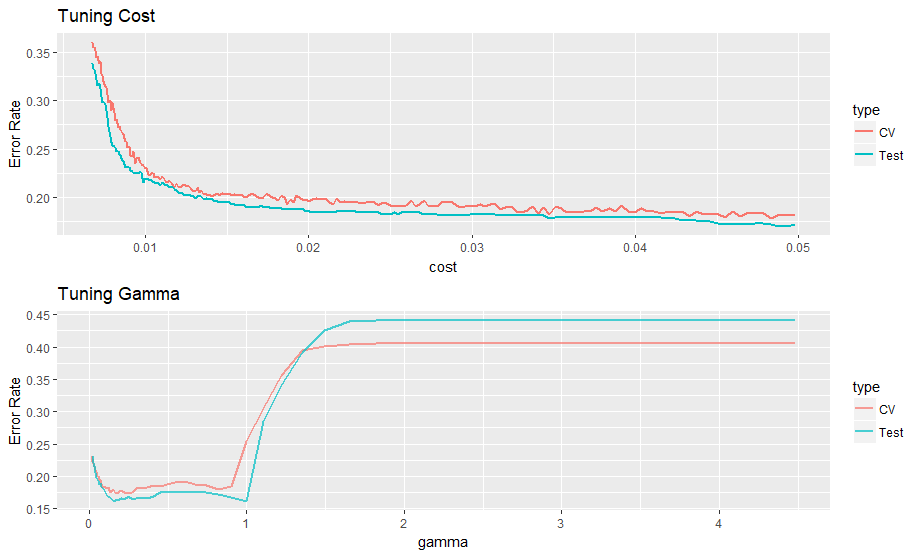
\includegraphics[width = .8\textwidth]{svm.png}
\caption{Parameter Tuning of SVM}
\label{svm}
\end{figure}

Kernel support vector machines (SVMs) are supervised learning models with associated learning algorithms commonly used in classification.\cite{cristianini2000introduction}

The effectiveness of SVM depends on the selection of kernel, the kernel's parameters, and soft margin parameter C. A common choice is a Gaussian kernel, which has a single parameter $\gamma$. The best combination of C and $\gamma$ is often selected by a grid search with exponentially growing sequences of C and $\gamma$. Each combination of parameter choices is checked using cross validation, and the parameters with best cross-validation accuracy are picked. We can do this with function \emph{tune} given a list of C. In Figure \ref{svm} we can see the CV error and test error of SVM using different cost and gamma. The best C is 0.05 and the best $\gamma$ is 0.135.

With the parameters tunned we can conduct classfication. The test error are shown in Table \ref{tblsvm}. The Type \uppercase\expandafter{\romannumeral1} error is slightly larger than random forest, but Type \uppercase\expandafter{\romannumeral2} error is significantly lower than random forest. So SVM made less mistake in predicting raining days compared to random forest. This could partly be explained by the fact that this isn't a linearly separable case. 

\begin{table}[h]
\setlength{\belowcaptionskip}{5pt}
\caption{Confusion Matrix and Error Rates of SVM}
\label{tblsvm}
\centering
\renewcommand\arraystretch{1.5}
\begin{tabular}{rrrrr}
\hline
\hline
 & & \multicolumn{2}{c}{True Condition} & \\
\hline
 & & Non-Precipitation & Precipitation & \\
\cline{1-4}
\multirow{2}{*}{Prediction} & {Non-Precipitation} & 326 & 47 & \\
\cline{2-4}
&Precipitation&54&231&\\
\hline
&Error Rate & 0.142 & 0.169 & 0.1535\\
\cline{2-5}
& & Type \uppercase\expandafter{\romannumeral1} & Type \uppercase\expandafter{\romannumeral2} & Overall\\
\hline
\end{tabular}
\end{table}
\subsection{$k$-Nearest Neighbors}

The $k$-nearest neighbors algorithm ($k$-NN) is a nonparametric method commonly used for classification, where each object is classified by a vote among its $k$ nearest neighbors.\cite{altman1992introduction} Since the algorithm is substantially a local method, it would be less likely to be influenced by global topology of the attribute space, which suggests an important advantage of applying $k$-NN here.

However, it is also noteworthy that the $k$-NN algorithm suffers from severe curse of dimensionality. What makes it worse is that we have got only 2192 observations here but more than 10 attributes. Therefore some variable selection must be applied before launching the $k$-NN algorithm.

\begin{figure}[h]
\center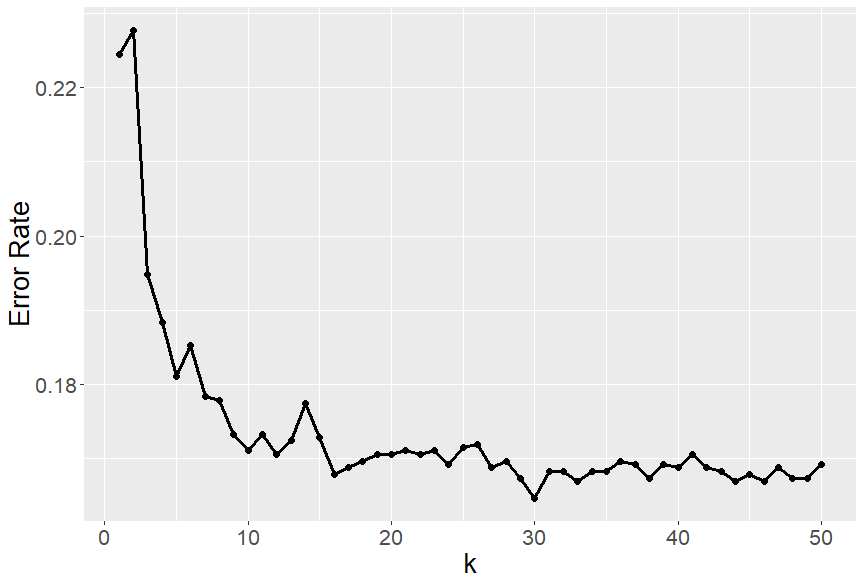
\includegraphics[width = .7\textwidth]{knncv.png}
\caption{Cross Validation Error Rates of \(k\)-NN}
\label{knncv}
\end{figure}

\begin{table}[h]
\setlength{\belowcaptionskip}{5pt}
\caption{Confusion Matrix and Error Rates of \(k\)-NN}
\label{errknn}
\centering
\renewcommand\arraystretch{1.5}
\begin{tabular}{rrrrr}
\hline
\hline
 & & \multicolumn{2}{c}{True Condition} & \\
\hline
 & & Non-Precipitation & Precipitation & \\
\cline{1-4}
\multirow{2}{*}{Prediction} & {Non-Precipitation} & 308 & 52 & \\
\cline{2-4}
&Precipitation&58&241&\\
\hline
&Error Rate & 0.1585 & 0.1775 & 0.1669\\
\cline{2-5}
& & Type \uppercase\expandafter{\romannumeral1} & Type \uppercase\expandafter{\romannumeral2} & Overall\\
\hline
\end{tabular}
\end{table}

Fortunately, the process of variable selection can be done with the result of the random forest which we have launched before. According to random forest, the most important attributes are PRCP, TDIF, and the four attributes regarding wind.

The data set can be even further reduced as we observe the strong correlation between WSF2 and WSF5 (their correlation turns out to be approximately $0.95$). Because of such stong colinearity, we would only keep 4 attributes, i.e. PRCP, TDIF, WSF5 and WDF5 in the $k$-NN algorithm. (Note that for wind vectors, the distances shall not be Euclidean as they are presented in polar coordinates.)

The cross validation error rates for different values of $k$ are shown above in Figure \ref{knncv}, which suggests that $k=30$ would be the best to proceed with. Then the confusion matrix and the test errors are as follows in Table \ref{errknn}.

As we can see, in general, SVM has the best performance, while $k$-NN the worse. It is also noteworthy that for all of the three methods here, there are always more Type \uppercase\expandafter{\romannumeral2} error than Type \uppercase\expandafter{\romannumeral1} error.


\subsection{Applying Models to New York City}

So what about applying the same models to climate data of a different city? We consider to use the weather data from New York City in 2017 as test data with the models trained by Seattle data. The same data preprocessing approach is followed as what we did on Seattle data. After that, we only apply SVM and random forest here as they have better performance than $k$-NN. The confusion matrices are shown respectively in Table \ref{ny1} and Table \ref{ny2}.

For random forest, the Type \uppercase\expandafter{\romannumeral1} error is significantly higher. Although the Type \uppercase\expandafter{\romannumeral2} error is lower, it is actually due to the model classified to many days into rain days mistakenly. The model predicted 289 days that rain in 2017 and the average raining day in New York based on historical record is 122. Overall, this model trained with Seattle data is not suitable to predict precipitation in New York. Again, we apply SVM with whole Seattle data as training set and test on New York. As shown in Table \ref{ny2}, the Type \uppercase\expandafter{\romannumeral1} error is significantly higher as well as the Type \uppercase\expandafter{\romannumeral2} error. Overall those two model performed badly in the New York data.

\begin{table}[h]
\setlength{\belowcaptionskip}{5pt}
\caption{Confusion Matrix for New York, Random Forest}
\label{ny1}
\centering
\renewcommand\arraystretch{1.5}
\begin{tabular}{rrrrr}
\hline
\hline
 & & \multicolumn{2}{c}{True Condition} & \\
\hline
 & & Non-Precipitation & Precipitation & \\
\cline{1-4}
\multirow{2}{*}{Prediction} & {Non-Precipitation} & 62 & 13 & \\
\cline{2-4}
&Precipitation&176&113&\\
\hline
&Error Rate & 0.7394 & 0.1031 & 0.5192\\
\cline{2-5}
& & Type \uppercase\expandafter{\romannumeral1} & Type \uppercase\expandafter{\romannumeral2} & Overall\\
\hline
\end{tabular}
\end{table}

\begin{table}[h]
\setlength{\belowcaptionskip}{5pt}
\caption{Confusion Matrix for New York, SVM}
\label{ny2}
\centering
\renewcommand\arraystretch{1.5}
\begin{tabular}{rrrrr}
\hline
\hline
 & & \multicolumn{2}{c}{True Condition} & \\
\hline
 & & Non-Precipitation & Precipitation & \\
\cline{1-4}
\multirow{2}{*}{Prediction} & {Non-Precipitation} & 96 & 45 & \\
\cline{2-4}
&Precipitation&142&81&\\
\hline
&Error Rate & 0.596 & 0.357 & 0.5137\\
\cline{2-5}
& & Type \uppercase\expandafter{\romannumeral1} & Type \uppercase\expandafter{\romannumeral2} & Overall\\
\hline
\end{tabular}
\end{table}

There are several possible explanations for this. First, New York located on the east coast may have totally different meteorological environment compares to Seattle. So the variables and the threshold of those variables that matter in prediction may change. Second, New York has a rather imbalanced situation which has more days without precipitation (in fact, 126 days with precipitation, and 238 days without).

\section{Conclusions}

After applying three methods, $k$-NN, SVM, random forest, to Seattle climate dataset, SVM and random forest have similar results in terms of overall error rate and are better than $k$-NN. SVM has a kind of balance between type \uppercase\expandafter{\romannumeral1} and type \uppercase\expandafter{\romannumeral2} error, while random forest has larger type \uppercase\expandafter{\romannumeral2} error and lower type \uppercase\expandafter{\romannumeral1} error. So random forest may make more mistakes in predicting days with precipitation. In reality people may care more and change their action, like bring an umbrella, if they know it will rain tomorrow. So in that case SVM would be better than random forest. Also the results of applying the model to New York data suggest we can’t use the models directly on another city without modification. Overall, the classification methods are reliable if we have enough history data and just want to make prediction of precipitation. 
 \vspace{3cm}
\bibliography{ref}
\addcontentsline{toc}{section}{Reference}

\end{document}


